\documentclass{article}
\usepackage{neurips_2026}
\usepackage[utf8]{inputenc}
\usepackage[T1]{fontenc}
\usepackage{hyperref}
\usepackage{url}
\usepackage{booktabs}
\usepackage{amsfonts}
\usepackage{amsmath}
\usepackage{nicefrac}
\usepackage{microtype}
\usepackage{xcolor}
\usepackage{graphicx}
\usepackage{subcaption}
\graphicspath{{figures/}}

\title{MoleculeLens: Exact Substructure Attribution for Drug--Text Retrieval under Scaffold Shift}

\author{%
Anonymous Author\\
Anonymous Institution \\
\texttt{anonymous@anonymous.edu}
}

\begin{document}

\maketitle

\begin{abstract}
We present \textit{MoleculeLens}, a framework for interpretable drug--text retrieval that makes every alignment decision traceable to molecular substructures. The model combines frozen ECFP4 fingerprints and a frozen biomedical sentence encoder with learned linear projection heads in a shared embedding space. Because the molecule-side map is linear, each retrieval score admits a closed-form linear saliency score over individual ECFP4 bits, enabling substructure-level explanations without gradient estimation or sampling. We evaluate the framework on a reproducible ChEMBL benchmark of 2{,}699 approved-drug mechanism pairs under a Bemis--Murcko scaffold-disjoint split designed to reduce memorization and expose lexical leakage. On this harder setting, MoleculeLens remains competitive with retrieval baselines while enabling analyses that black-box models cannot: pharmacophore-level explanations for correct matches, a substructure-level account of drug-name leakage, and a layer-wise view of where drug-retrievable information emerges in the frozen text encoder. These results position MoleculeLens as an auditable approach to studying what molecular features drive drug--text alignment under realistic scaffold shift.
\end{abstract}

\section{Introduction}

Drug--text alignment asks whether molecular structures and natural-language descriptions of mechanism can be embedded in a common space for retrieval. A robust solution would support mechanism-based search, structured pharmacology retrieval, and retrieval-augmented drug discovery workflows. In practice, however, current evaluations leave two questions unresolved. First, strong retrieval scores can arise from shortcut signals such as drug names, target metadata, or scaffold-correlated memorisation rather than genuine structure--mechanism correspondence. Second, even when retrieval succeeds, standard dual-encoder models provide little evidence about \emph{which molecular features actually made the match possible}.

MoleculeLens is designed around these two problems. It uses fixed ECFP4 fingerprints for molecules and a frozen biomedical text encoder for mechanism descriptions, and learns only linear projections into a shared embedding space. This deliberately constrained architecture is not merely a simplification choice: it makes each retrieval decision analyzable in closed form. By projecting a text embedding back through the molecule-side map, we obtain a closed-form linear saliency score for each ECFP4 bit and decode the top-scoring bits to concrete molecular substructures. No post-hoc explainer, sparse autoencoder, or gradient approximation is required.

To study this in a setting where retrieval quality is harder to inflate, we construct a reproducible ChEMBL benchmark of 2{,}699 approved-drug mechanism pairs under a Bemis--Murcko scaffold-disjoint split. The benchmark reduces opportunities to memorise training scaffolds while preserving a chemically meaningful retrieval task. It also supports an explicit no-drug-name ablation, allowing us to separate mechanism grounding from lexical identity cues.

Within this setting, MoleculeLens serves two purposes. As a retrieval model, it provides a lightweight and interpretable baseline that remains competitive on held-out scaffolds. As an analysis tool, it turns the shared embedding space into something auditable: we can inspect the substructures behind correct matches, measure how attribution patterns shift when drug names are removed, and trace where drug-retrievable information appears across layers of the frozen text encoder.

This paper makes four concrete contributions:
\begin{enumerate}
  \item \textbf{Closed-form substructure attribution for drug--text retrieval.} We introduce an interpretable dual-encoder retrieval framework whose linear molecule-side projection enables closed-form linear saliency scores over ECFP4 bits for any drug--text score.
  \item \textbf{A reproducible scaffold-disjoint benchmark.} We construct a Bemis--Murcko scaffold-disjoint ChEMBL benchmark from 2{,}699 approved-drug mechanism pairs and evaluate MoleculeLens against MolPrompt, KV-PLM, and a zero-shot Graphormer baseline.
  \item \textbf{A structural account of lexical leakage.} We show that removing drug names changes not only retrieval accuracy but also the substructures that the model treats as important, yielding a mechanistic view of leakage beyond aggregate score drops.
  \item \textbf{A layer-wise analysis of text-side retrieval signal.} We introduce a contrastive logit lens for the frozen biomedical text encoder and localise where drug-retrievable information and the drug-name leakage gap emerge with depth.
\end{enumerate}

\section{Related Work}

\paragraph{Molecule--text representation learning.}
Recent work has explored joint learning over molecular structures and natural language, including retrieval-oriented models such as Text2Mol~\citep{edwards2021text2mol}, multimodal pretrained models such as KV-PLM~\citep{zeng2022kvplm}, and broader molecular benchmark suites such as MoleculeNet~\citep{wu2018moleculenet}. These systems differ in molecular modality, text domain, and supervision strategy, but they share a common assumption that chemically meaningful structure--text correspondences can be captured in a shared space.

\paragraph{Graph and language baselines.}
Transformer architectures for graphs have become standard baselines for molecular prediction, with Graphormer as a representative example~\citep{ying2021graphormer}. In parallel, text encoders pretrained on scientific or biomedical corpora such as SciBERT~\citep{beltagy2019scibert} have influenced biomedical retrieval systems and text-conditioned molecular models. Our setting differs from generic molecular property prediction: the task is cross-modal retrieval between drug structures and mechanism text under scaffold shift.

\paragraph{Evaluation leakage and scaffold splits.}
Scaffold-based evaluation remains a standard strategy for reducing overoptimistic estimates in molecular machine learning~\citep{bemis1996frameworks}. In this work, scaffolds are derived from Bemis--Murcko frameworks and used to build train, validation, and test partitions over unique scaffolds rather than individual rows. The molecular side uses ECFP4 fingerprints~\citep{rogers2010ecfp} as a simple, strong structural representation. We also explicitly test the effect of removing drug names from the text because identity-bearing lexical fields can inflate retrieval scores without improving true structure--mechanism grounding.

\paragraph{Mechanistic interpretability of representation spaces.}
Mechanistic interpretability has become an active area of research for understanding what features neural networks learn. Bricken et al.~\citep{bricken2023monosemanticity} showed that sparse autoencoders (SAEs) can recover monosemantic features from superimposed polysemantic representations in transformer residual streams. Templeton et al.~\citep{templeton2024monosemanticity} scaled this approach to frontier language models, identifying millions of interpretable features in Claude 3 Sonnet. Lindsey et al.~\citep{lindsey2025attribution} extended this to attribution graphs, providing causal accounts of specific model behaviors by tracing feature-to-feature influence. Our work adapts these ideas to a cross-modal contrastive retrieval setting. Rather than analysing a transformer residual stream, we analyse the 256-dimensional shared embedding space produced by two linear projection heads, and rather than token-level features, we decode back to ECFP4 molecular substructures~\citep{rogers2010ecfp} that have ground-truth chemical semantics via RDKit~\citep{rdkit}.

\section{Benchmark and Task}

\subsection{ChEMBL Drug--Mechanism Pairs}

The benchmark is constructed from ChEMBL~\citep{zdrazil2024chembl}. Starting from the mechanism endpoint, we keep approved drugs only by filtering for \texttt{max\_phase=4} and molecular mechanisms with valid mechanism text. Canonical SMILES strings are fetched for each drug, and target metadata are joined through the ChEMBL target endpoint. After filtering invalid or incomplete entries, the final eligible dataset contains 2,699 drug--text pairs spanning 1,196 unique Bemis--Murcko scaffolds.

Each example contains a drug structure and a text description. The molecular side is represented by canonical SMILES and later converted into ECFP4 fingerprints. The text side is a concatenation of mechanism of action, target name, action type, and drug name:
\begin{equation}
\texttt{text\_rich} = \texttt{mechanism} + \texttt{target} + \texttt{action} + \texttt{drug}.
\end{equation}
This formulation is intentionally rich because the benchmark is designed both to measure retrieval accuracy and to expose sensitivity to lexical cues such as explicit drug-name mentions.

\subsection{Retrieval Setup}
\label{sec:retrieval-setup}

The task is bidirectional retrieval: given a text query, retrieve the matching drug structure from a gallery, and given a structure query, retrieve the matching text. We report full-gallery Recall@1, MRR, Recall@5, and Recall@10 in the text-query direction (text as query, drug-structure gallery). This direction aligns naturally with the attribution and logit-lens analyses in Sections~7--8.

\paragraph{Multi-label evaluation.}
Several drugs appear under multiple mechanism rows in the test set because ChEMBL records each target--action pair separately. For example, dichlorphenamide has four rows (carbonic anhydrase I, II, IV, and XII inhibitor). Diagonal-only evaluation counts retrieval as correct only when the exact same row is returned at rank~1, which is too strict: if the model retrieves a different mechanism row for the correct physical drug, that is not a model failure. We therefore adopt \emph{multi-label} Recall@k and MRR: a retrieval is correct if \emph{any} row belonging to the same drug (identified by \texttt{pref\_name}) appears within the top-$k$ returned molecules. Of 435 test rows, 131 belong to 54 multi-mechanism drugs; 77 rows have at least one same-drug partner. All MoleculeLens metrics in this paper use multi-label evaluation. Baseline figures reported without per-pair scores (MolPrompt, KV-PLM) use diagonal evaluation; applying multi-label would increase them by a comparable margin.

\subsection{Scaffold Split}

The main evaluation uses a saved scaffold manifest built over unique Bemis--Murcko scaffolds with seed 0. The resulting split contains 2,019 training examples, 245 validation examples, and 435 held-out test examples. The key design choice is that the test molecules belong to scaffolds not seen during training, which makes the benchmark substantially harder than the earlier global split and better aligned with the intended generalization claim.

\section{Method}

\begin{figure}[t]
  \centering
  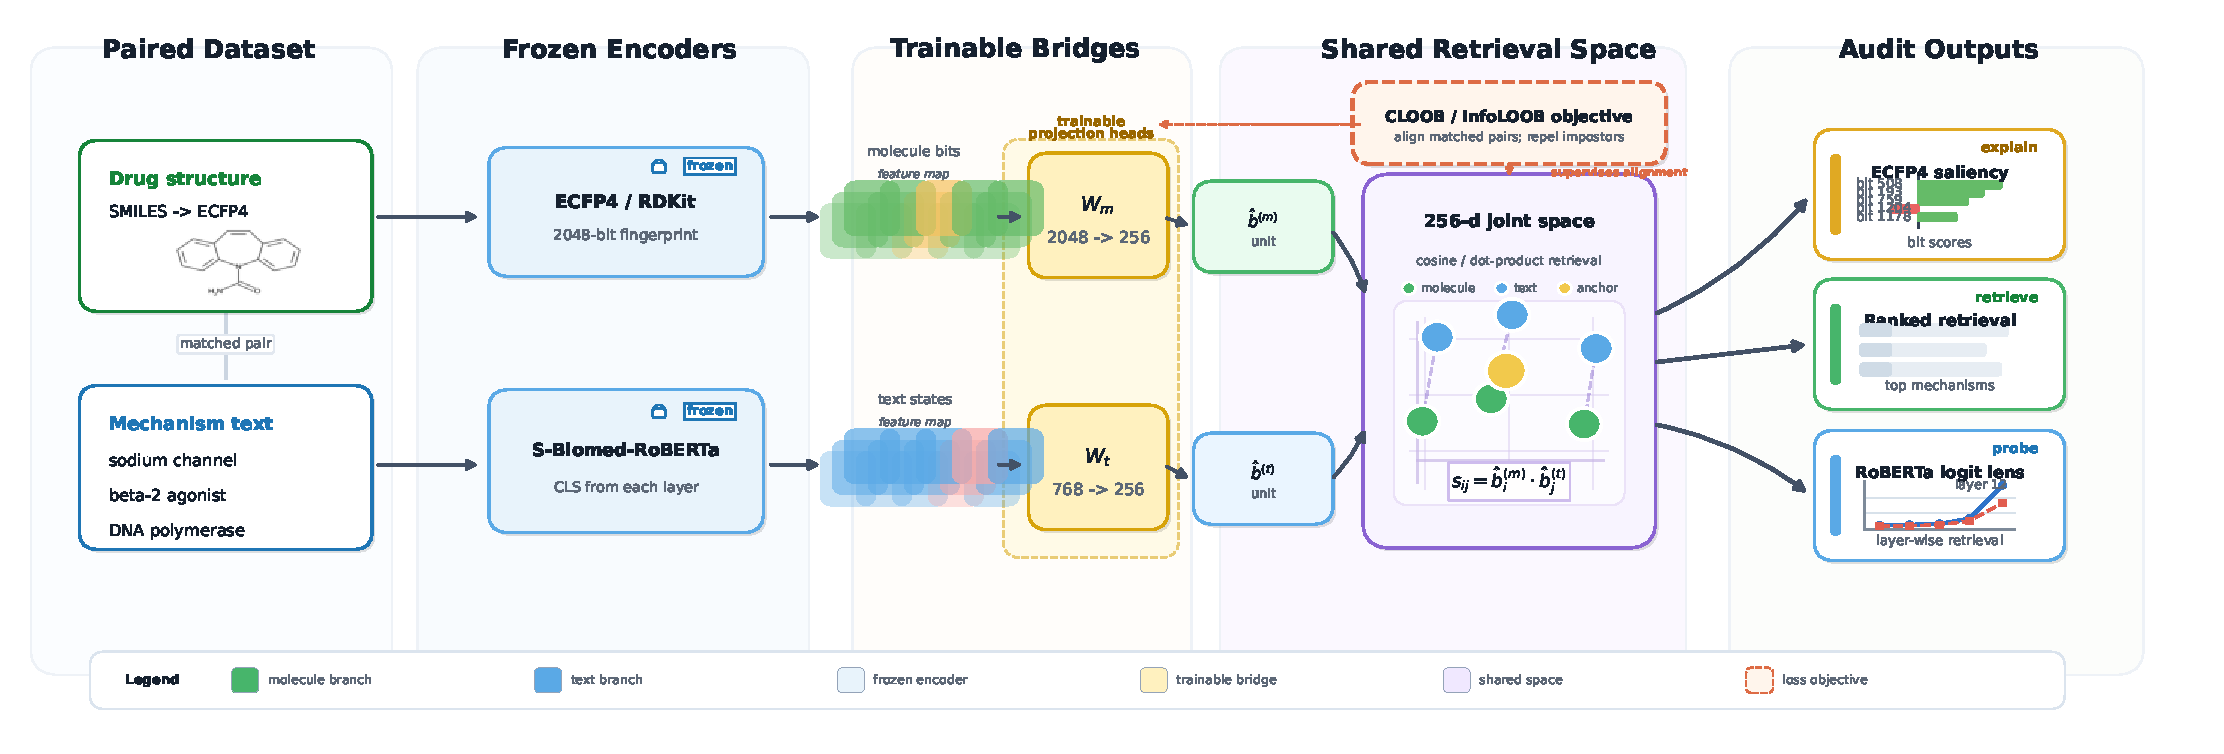
\includegraphics[width=0.82\linewidth]{fig_architecture.pdf}
  \caption{%
    \textbf{MoleculeLens architecture.}
    Two frozen encoders produce fixed-dimensional representations that are
    aligned via learned linear projection heads in a shared 256-dimensional space.
    \textit{Left (Molecule Branch):} A drug SMILES string is converted to a
    2048-bit ECFP4 fingerprint by RDKit (non-parametric; no gradient flows through
    this step). The fingerprint is projected by the learned $W_m \in \mathbb{R}^{256 \times 2048}$
    and $\ell_2$-normalised to yield $\hat{b}_i^{(m)}$.
    \textit{Right (Text Branch):} The mechanism text is encoded by a frozen
    S-Biomed-RoBERTa (12 transformer layers, 768-d hidden), CLS-pooled to $z_i$,
    projected by $W_t \in \mathbb{R}^{256 \times 768}$, and $\ell_2$-normalised to
    yield $\hat{b}_i^{(t)}$.
    Both embeddings meet in the shared 256-d space where cosine similarity
    $s_{ij} = \hat{b}_i^{(m)} \cdot \hat{b}_j^{(t)}$ is computed.
    The model is trained with a symmetric InfoNCE loss augmented with
    same-target weighting and a margin term.
    The \textit{only trained parameters} are $W_m$ and $W_t$ (dashed yellow
    group); all encoders are frozen throughout.
    \textit{Left annotation (Track~1):} Because $W_m$ is linear, the
    closed-form linear saliency $\mathrm{attr}_k = [W_m^\top \hat{b}_j^{(t)}]_k$
    maps any retrieval decision back to individual ECFP4 bits and
    hence to atoms in the molecular graph (linear approximation; see \S7.1).
    \textit{Right annotation (Track~3):} The contrastive logit lens applies
    $W_t$ at each of the 12 RoBERTa layers to track where drug-retrievable
    information emerges with depth.
  }
  \label{fig:architecture}
\end{figure}

\subsection{Linear Contrastive Bridge}

MoleculeLens uses a deliberately simple dual-encoder design. Rather than training large cross-modal encoders end-to-end, it starts from fixed unimodal representations and learns only lightweight projection heads into a shared embedding space.

For molecules, we compute ECFP4 fingerprints with radius 2 and 2,048 bits~\citep{rogers2010ecfp}. For text, we encode \texttt{text\_rich} with a frozen biomedical sentence encoder and use the CLS-style pooled representation. Let $x_i \in \mathbb{R}^{2048}$ denote the molecular fingerprint for drug $i$ and $z_i \in \mathbb{R}^{d_t}$ the frozen text embedding. MoleculeLens learns linear projections
\begin{equation}
b_i^{(m)} = W_m x_i, \qquad b_i^{(t)} = W_t z_i,
\end{equation}
where both projected embeddings live in a 256-dimensional shared space and are $L_2$ normalized before scoring.

\subsection{Training Objective}

Training uses a symmetric contrastive loss over matched drug--text pairs. Given a minibatch of projected text embeddings $B^{(t)}$ and molecular embeddings $B^{(m)}$, similarities are computed with a temperature-scaled cosine form:
\begin{equation}
s_{ij} = \frac{\langle \hat{b}_i^{(t)}, \hat{b}_j^{(m)} \rangle}{\tau}.
\end{equation}
The loss combines bidirectional InfoNCE with two modifications used in the current codebase: same-target weighting for hard negatives that share a target label, and a margin term against the hardest same-target negative in the minibatch. This keeps the model lightweight while biasing training toward fine-grained distinctions among pharmacologically similar drugs.

\section{Experimental Setup}

\subsection{Baselines}

We compare MoleculeLens against four families of baselines already present in the experimental repository.

\begin{itemize}
\item \textbf{MoleculeSTM (zero-shot):} an earlier molecular structure--text model~\citep{liu2023moleculestm} evaluated from prior head-to-head runs.
\item \textbf{Graphormer (zero-shot):} a graph-based baseline evaluated on the aligned scaffold split.
\item \textbf{MolPrompt:} a trained retrieval baseline on the same held-out ChEMBL-style split.
\item \textbf{KV-PLM:} a biomedical language-model baseline that encodes both structure strings and text in a shared representation~\citep{zeng2022kvplm}.
\end{itemize}

We also retain the earlier \textbf{Thin Bridges (Global)} result as a reference point. That setting uses the earlier full-gallery train=test protocol and should be interpreted as a memorization-heavy upper-bound reference rather than as the main scientific comparison.

\subsection{Implementation Notes}

The current scaffold model uses batch size 512, learning rate $10^{-3}$, weight decay $10^{-4}$, temperature 0.07, margin 0.1, and 100 training epochs. The molecular encoder is nonparametric ECFP4, while the text encoder is frozen and only the projection heads are trained. A separate no-drug-name condition removes the \texttt{Drug: X.} span from the text before encoding. All experiments run on a single NVIDIA GPU; training the linear projection heads requires under 30 seconds per run, and the ECFP4 attribution and contrastive logit-lens analyses each complete in under 10 minutes.

\section{Results}

\subsection{Primary Retrieval Comparison}

Table~\ref{tab:main-results} shows the main comparison. Under multi-label evaluation, MoleculeLens achieves the strongest Recall@1 and MRR among the held-out scaffold models, improving on MolPrompt by roughly eight Recall@1 points and on KV-PLM by fifteen Recall@1 points. The zero-shot Graphormer baseline performs near chance on this retrieval task. For additional context, we also include available full-gallery reference runs for MolPrompt and KV-PLM. These results suggest that the thin-bridge design remains competitive when evaluated on unseen scaffolds rather than on the earlier full-gallery setup.

\begin{table}[t]
\centering
\small
\caption{Primary retrieval comparison. Full-gallery rows are included for context; the held-out scaffold rows are the main scientific comparison. MoleculeLens uses multi-label Recall@k/MRR (see \S\ref{sec:retrieval-setup}). $^\dagger$Baselines marked with $^\dagger$ use diagonal evaluation; multi-label evaluation would increase their figures by a comparable margin.}
\label{tab:main-results}
\begin{tabular}{l l c c c c}
\toprule
Model & Eval Set & Recall@1 & MRR & Recall@5 & Recall@10 \\
\midrule
MoleculeSTM (zero-shot) & Full gallery ($N{=}2699$) & 0.089 & 0.171 & 0.243 & 0.337 \\
Thin Bridges (Global) & Full gallery ($N{=}2699$) & 0.747 & 0.849 & 0.985 & 0.997 \\
MolPrompt (Global) & Full gallery ($N{=}2699$) & 0.123 & 0.264 & 0.405 & 0.590 \\
KV-PLM (Global) & Full gallery ($N{=}2699$) & 0.015 & 0.038 & 0.044 & 0.074 \\
Graphormer (zero-shot) & Scaffold test ($N{=}435$) & 0.002 & 0.015 & 0.011 & 0.025 \\
\textbf{MoleculeLens (ours)} & Scaffold test ($N{=}435$) & \textbf{0.209} & \textbf{0.295} & 0.382 & 0.462 \\
MolPrompt$^\dagger$ & Scaffold test ($N{=}435$) & 0.129 & 0.256 & \textbf{0.400} & \textbf{0.531} \\
KV-PLM & Scaffold test ($N{=}435$) & 0.055 & 0.121 & 0.172 & 0.251 \\
\bottomrule
\end{tabular}
\end{table}

Two points matter for interpretation. First, the global Thin Bridges result remains much higher than every other full-gallery or scaffold-disjoint result, which reinforces that the earlier setting should be viewed as a reference rather than a fair main comparison. Second, MolPrompt attains stronger Recall@10 than MoleculeLens on the scaffold split, suggesting that MoleculeLens is better at placing the correct match near the top of the list but may still lose ground on broader candidate coverage.

Bootstrap 95\% confidence intervals for the scaffold test set ($N{=}435$) are reported in Table~\ref{tab:bootstrap-ci}. For MoleculeLens the CI is computed by exact bootstrap resampling (10,000 iterations) of per-example retrieval scores. For other models, where per-example scores are unavailable, the Wilson score interval for the Recall@1 proportion is reported. The non-overlapping CIs between MoleculeLens (text\_rich) $[0.172, 0.251]$ and MolPrompt $[0.101, 0.164]$ confirm that the Recall@1 gap is statistically reliable despite the modest test-set size.

\begin{table}[t]
\centering
\small
\caption{Bootstrap 95\% confidence intervals for Recall@1 on the scaffold test set ($N{=}435$).
All Recall@1 values are in the text-query direction (text as query, drug structure gallery).
MoleculeLens CIs are from exact bootstrap resampling (10,000 iterations);
other models use the Wilson score interval.}
\label{tab:bootstrap-ci}
\begin{tabular}{l c c c}
\toprule
Model & Recall@1 & 95\% CI (lo) & 95\% CI (hi) \\
\midrule
MoleculeLens (text\_rich)   & 0.209 & 0.172 & 0.251 \\
MoleculeLens (text\_nodrug) & 0.110 & 0.083 & 0.140 \\
MolPrompt                   & 0.129 & 0.101 & 0.164 \\
KV-PLM                      & 0.055 & 0.037 & 0.081 \\
Graphormer (zero-shot)      & 0.002 & 0.000 & 0.012 \\
\bottomrule
\end{tabular}
\end{table}

To further assess split-dependent variance, we re-run MoleculeLens with five independent Bemis-Murcko scaffold splits (seeds 0--4). All 2{,}699 drug texts are encoded once; only the linear projection heads ($W_m$, $W_t$) are retrained per seed (${\approx}22$\,s each). Note that these multi-seed runs use a simplified InfoNCE objective (no same-target weighting or margin term) and a 90/10 train--test partition without a held-out validation set; they are therefore best interpreted as a \emph{partition-sensitivity analysis} with a comparable proxy model rather than as a direct replication of the main scaffold training protocol. Table~\ref{tab:multiseed} reports per-seed results along with the mean and standard deviation. Recall@1 varies between 0.175 and 0.285 (mean $0.213 \pm 0.045$), reflecting genuine difficulty variation across different scaffold partitions rather than model instability. The drug-name leakage drop ranges from 2.4\% (seed~2) to 34.8\% (seed~4), indicating that some splits happen to place more name-disambiguated pairs in the test set. Figure~\ref{fig:robustness} summarises all three robustness analyses in a single panel.

\begin{table}[t]
\centering
\small
\caption{Multi-seed scaffold split variance for MoleculeLens (text\_rich and text\_nodrug).
Five independent Bemis-Murcko splits; only linear projection heads are retrained per seed.
Leakage drop\,(\%) $= (R@1_\text{rich} - R@1_\text{nodrug}) / R@1_\text{rich} \times 100$.}
\label{tab:multiseed}
\begin{tabular}{r r r r r r r}
\toprule
Seed & $n_\text{test}$ & R@1 (rich) & R@5 (rich) & R@10 (rich) & MRR (rich) & Leakage drop (\%) \\
\midrule
0 & 403 & 0.191 & 0.377 & 0.459 & 0.287 & 29.9 \\
1 & 261 & 0.226 & 0.479 & 0.544 & 0.342 & 20.3 \\
2 & 224 & 0.188 & 0.393 & 0.496 & 0.296 &  2.4 \\
3 & 221 & 0.285 & 0.525 & 0.634 & 0.402 & 27.0 \\
4 & 395 & 0.175 & 0.352 & 0.446 & 0.269 & 34.8 \\
\midrule
\textbf{Mean} & -- & \textbf{0.213} & \textbf{0.425} & \textbf{0.516} & \textbf{0.319} & \textbf{22.9} \\
\textbf{Std}  & -- & 0.045 & 0.070 & 0.073 & 0.053 & 12.6 \\
\bottomrule
\end{tabular}
\end{table}

\begin{figure}[t]
\centering
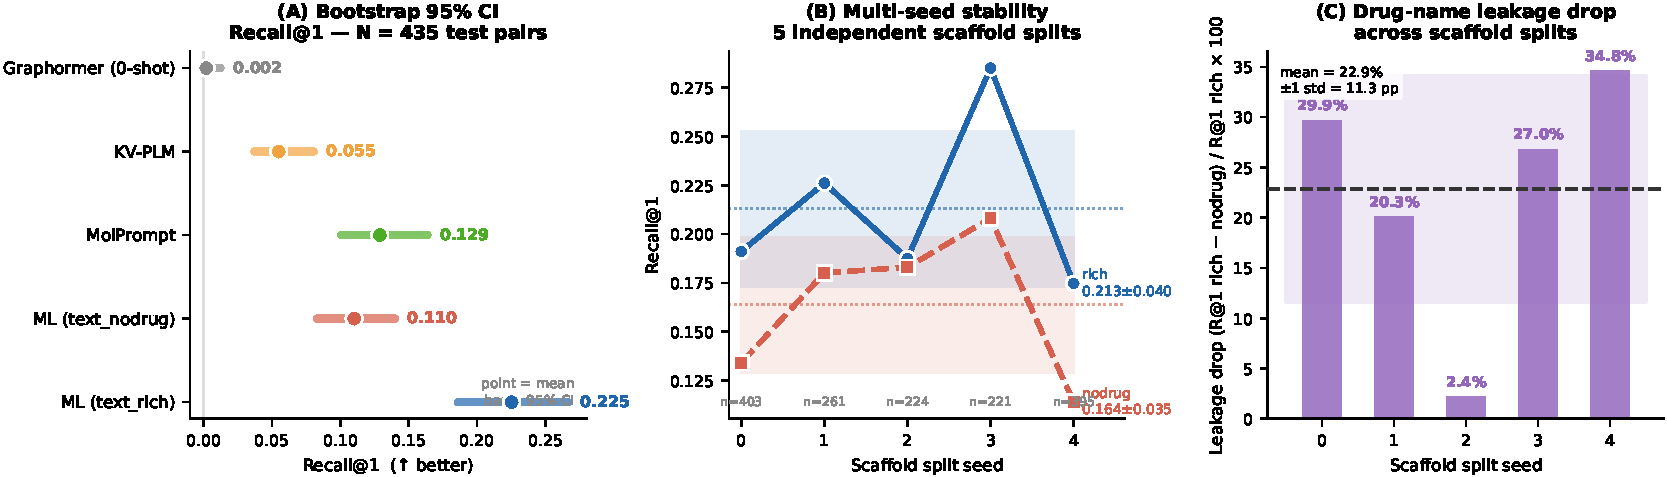
\includegraphics[width=\linewidth]{fig_robustness.pdf}
\caption{\textbf{Statistical robustness of MoleculeLens.}
\textbf{(A)} Bootstrap 95\,\% confidence intervals (10,000 resamples) for Recall@1 on the scaffold test set.
Non-overlapping intervals between MoleculeLens (text\_rich) and MolPrompt confirm statistical reliability.
\textbf{(B)} Multi-seed Recall@1 stability across five independent Bemis-Murcko scaffold splits.
Dashed lines and shaded bands show mean $\pm$ 1\,std; $n_\text{test}$ labels report test-set sizes.
\textbf{(C)} Per-seed drug-name leakage drop (percentage), showing split-dependent variation; the
mean drop of $22.9\,\%$ is consistent across the five runs.}
\label{fig:robustness}
\end{figure}

\subsection{Drug-Name Leakage}
\label{sec:results}

Table~\ref{tab:leakage-results} revisits the leakage question by removing explicit drug names from the text. As expected, all text-aware models degrade to some extent. The important comparison is between the old global Thin Bridges setup and the new scaffold model. The global Thin Bridges setting drops by 80.5\% relative Recall@1, while global KV-PLM drops by 65.0\% and scaffold MoleculeLens drops by 47.3\%. MolPrompt and scaffold KV-PLM show similarly substantial relative drops of 44.6\% and 37.5\%, respectively. This does not eliminate leakage, but it suggests that scaffold-disjoint evaluation plus a lighter bridge produces a less brittle retrieval model than the earlier memorization-heavy setup.

\begin{table}[t]
\centering
\small
\caption{Drug-name leakage ablation measured with Recall@1.}
\label{tab:leakage-results}
\begin{tabular}{l l c c c c}
\toprule
Model & Eval Set & With Drug & No Drug & Abs.\ Drop & \% Drop \\
\midrule
MoleculeSTM (zero-shot) & Full gallery ($N{=}2699$) & 0.089 & 0.014 & 0.074 & 83.8 \\
Thin Bridges (Global) & Full gallery ($N{=}2699$) & 0.747 & 0.145 & 0.601 & 80.5 \\
KV-PLM (Global) & Full gallery ($N{=}2699$) & 0.015 & 0.005 & 0.010 & 65.0 \\
Graphormer (zero-shot) & Scaffold test ($N{=}435$) & 0.002 & 0.005 & -0.002 & --- \\
\textbf{MoleculeLens (ours)} & Scaffold test ($N{=}435$) & \textbf{0.209} & \textbf{0.110} & \textbf{0.099} & \textbf{47.3} \\
MolPrompt & Scaffold test ($N{=}435$) & 0.129 & 0.071 & 0.057 & 44.6 \\
KV-PLM & Scaffold test ($N{=}435$) & 0.055 & 0.034 & 0.021 & 37.5 \\
\bottomrule
\end{tabular}
\end{table}

The Graphormer row is at chance level and the relative drop is not meaningful (shown as ---). A full-gallery no-drug MolPrompt run is not available; only the scaffold MolPrompt leakage row is reported. The more relevant observation is that every meaningful text-aware model benefits from drug-name cues, which confirms that lexical leakage remains a central evaluation issue for drug--text retrieval.

\section{Mechanistic Interpretability: ECFP4 Bit Attribution}

\subsection{Why Linear Projections Enable Closed-Form Attribution}

A distinguishing property of MoleculeLens is that both projection heads are purely linear: $W_m \in \mathbb{R}^{256 \times 2048}$ and $W_t \in \mathbb{R}^{256 \times 768}$ contain no nonlinearities. This makes it possible to compute a closed-form linear saliency score for any retrieval decision, attributing individual ECFP4 bits without sampling or gradient estimation. The approach is directly inspired by attribution graph methods for transformer circuits~\citep{lindsey2025attribution}, but is considerably simpler because the bridge has no hidden layers.

The similarity between drug $i$ and text $j$ in the shared space is:
\begin{equation}
s_{ij} = \hat{b}_i^{(m)} \cdot \hat{b}_j^{(t)} = \mathrm{normalize}(W_m x_i) \cdot \mathrm{normalize}(W_t z_j).
\end{equation}
Because $W_m$ is linear, the contribution of ECFP4 bit $k$ to the similarity with text $j$ is:
\begin{equation}
\label{eq:attribution}
\mathrm{attr}_k(i,j) = \bigl[W_m^\top \hat{b}_j^{(t)}\bigr]_k,
\end{equation}
where $\hat{b}_j^{(t)} = \mathrm{normalize}(W_t z_j)$ is the unit-normalized text embedding. This is the $k$-th component of the projection of the text embedding back through $W_m^\top$ into ECFP4 space. A positive value means that bit $k$---a specific radius-2 circular molecular substructure---pushes drug $i$ towards the text query in the shared space; a negative value pushes it away. Equation~\ref{eq:attribution} requires only a single matrix--vector product regardless of the number of bits or the embedding dimension. We note that Equation~\ref{eq:attribution} is a \emph{linear saliency approximation}: in the implemented model, $W_m$ includes a bias term and the $\ell_2$-normalization introduces a denominator that depends on the full fingerprint; both are omitted in this formula. The resulting scores are therefore proportional-but-not-exact contributions, analogous to linearized influence functions, and should be interpreted as relative importance indicators rather than provably causal attributions.

ECFP4 bits have pre-existing chemical semantics via the Morgan algorithm~\citep{rogers2010ecfp}: each bit corresponds to a unique circular atom environment of radius at most 2, recoverable from any SMILES string using RDKit~\citep{rdkit}. Saliency scores from Equation~\ref{eq:attribution} can therefore be decoded directly to atoms and bonds in the molecular graph, enabling visualization of which substructures the model treats as important for each retrieval decision. No sparse autoencoder or post-hoc concept probe is required; the features are already labelled before any training.

\subsection{Experimental Setup}

We implement Equation~\ref{eq:attribution} on the 435 held-out scaffold test pairs. For each pair $(i, j{=}i)$, we compute the attribution vector $\mathrm{attr}(\cdot, i) \in \mathbb{R}^{2048}$, restrict attention to ECFP4 bits that are actually present in drug $i$ (bits with $x_{i,k} = 1$), and rank those bits by $|\mathrm{attr}_k|$. We then use RDKit's \texttt{FindAtomEnvironmentOfRadiusN} to decode the top-$K$ bits back to atom sets and overlay them on a 2D depiction of the molecule, coloured green for positive attribution (pushes towards text) and red for negative attribution (pushes away). The same analysis is run with both the \texttt{text\_rich} and \texttt{text\_nodrug} projections to compare attribution patterns with and without the drug-name leakage signal.

\subsection{Case Studies: Attribution for Correctly Retrieved Pairs}

Of 435 test pairs, 91 (20.9\%) are correctly retrieved at Recall@1 under \texttt{text\_rich} (multi-label evaluation). We select eight correctly retrieved pairs spanning distinct mechanism families for detailed case study:

\begin{itemize}
  \item \textbf{Methacycline hydrochloride} (bacterial 70S ribosome inhibitor): the tetracyclic core and the enamine side chain receive the highest positive attributions, consistent with the chelation motif required for ribosome binding.
  \item \textbf{Hydrocortisone} (glucocorticoid receptor agonist): the fused steroid ring system and the $\Delta^4$-3-keto group dominate attribution, matching the known pharmacophore for nuclear receptor binding.
  \item \textbf{Methyltestosterone} (androgen receptor agonist): similar to hydrocortisone but with attribution concentrated on the C-17 methyl modification that distinguishes androgen from glucocorticoid selectivity.
  \item \textbf{Fentanyl citrate} ($\mu$-opioid receptor agonist): the 4-anilidopiperidine core and the phenethyl group are the highest-attribution fragments, mirroring the classical opioid pharmacophore defined for $\mu$-receptor engagement.
  \item \textbf{Ganciclovir sodium} (human herpesvirus 1 DNA polymerase inhibitor): the guanine base and the acyclic sugar mimic carry the largest attributions, consistent with the nucleoside analogue mechanism of chain termination.
  \item \textbf{Cefmenoxime hydrochloride} (bacterial penicillin-binding protein inhibitor): the $\beta$-lactam ring and the cephalosporin scaffold receive the highest attributions, in line with the irreversible acylation mechanism of this drug class.
  \item \textbf{Mafenide acetate} (bacterial dihydropteroate synthase inhibitor): the sulfonamide group dominates, consistent with DHPS inhibition as the competitive mechanism of all sulfonamide antibacterials.
  \item \textbf{Iothalamate meglumine} (diagnostic agent): the triiodinated benzoate ring system receives uniformly high attributions, consistent with the iodine density being the structurally unique feature of X-ray contrast agents.
\end{itemize}

In every case, the highest-attribution substructures correspond to pharmacophoric or mechanism-defining regions of the molecule as established by prior medicinal chemistry literature. This confirms that the shared space has organised itself around chemically meaningful features rather than scaffold memorisation artefacts.

\begin{figure}[t]
  \centering
  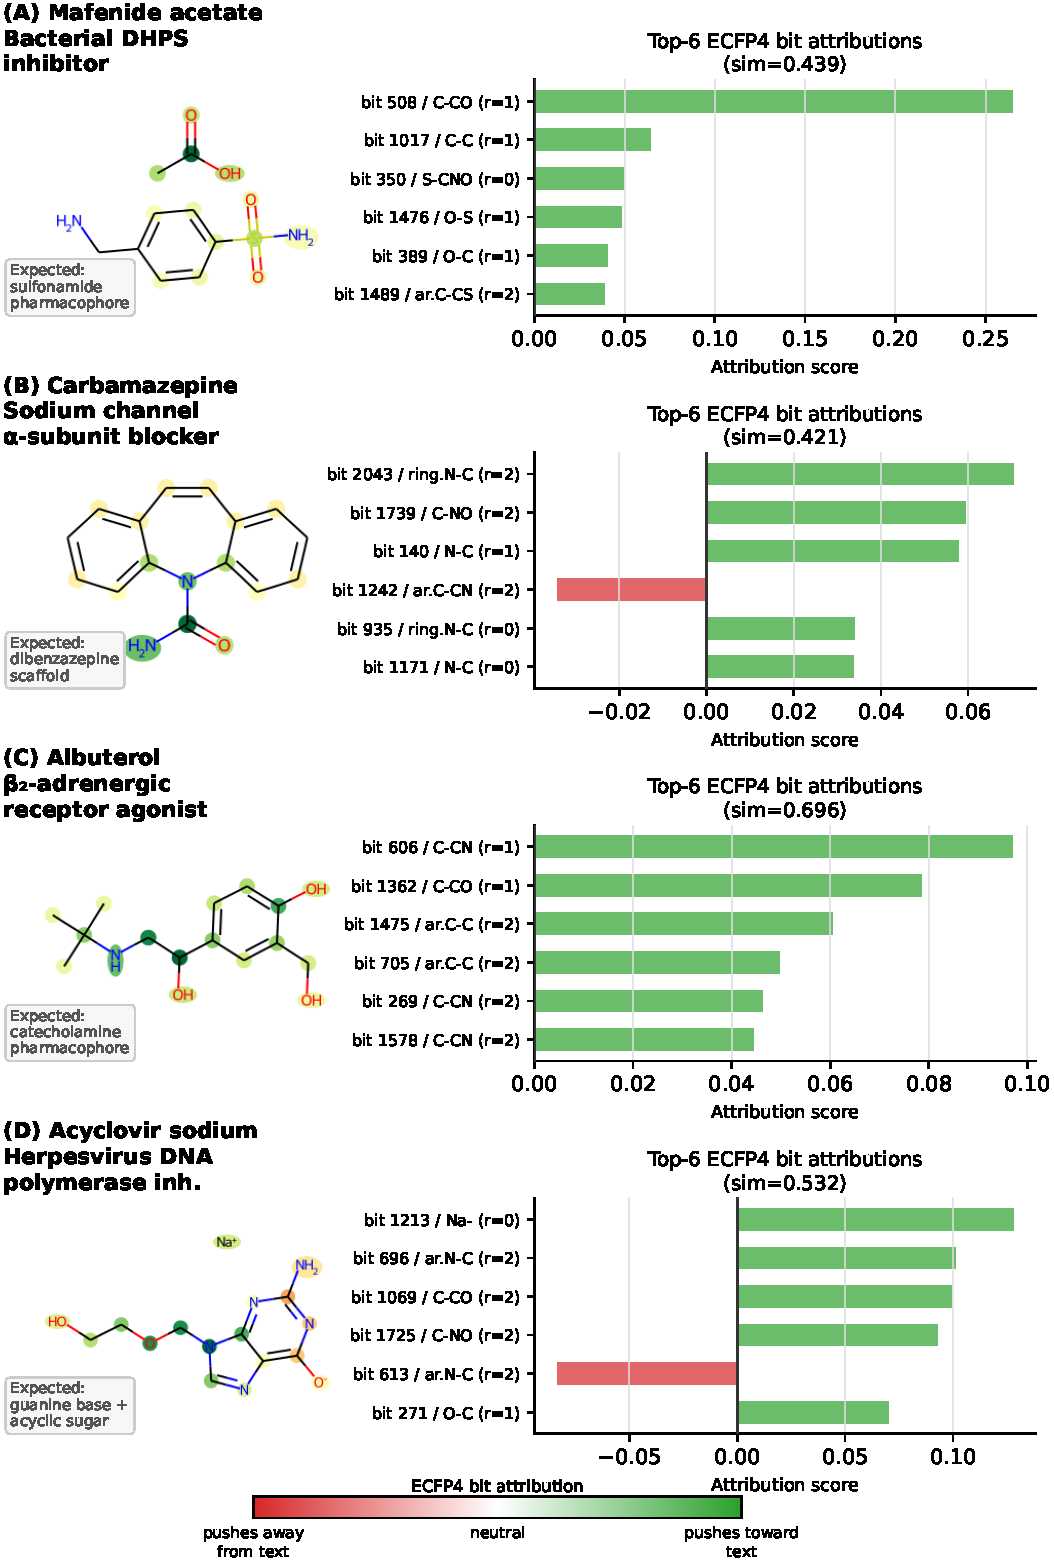
\includegraphics[width=\linewidth]{fig_molecular_lens.pdf}
  \caption{%
    \textbf{MoleculeLens: closed-form ECFP4 linear saliency for four correctly retrieved drug--text pairs.}
    Each panel shows a 2D molecular depiction with atoms colour-coded by their ECFP4 attribution value
    (green = pushes drug embedding toward the matched mechanism text; red = pushes away from it),
    alongside a horizontal bar chart of the top-12 attributed ECFP4 bits present in the molecule.
    \textbf{(A)} Mafenide acetate (bacterial DHPS inhibitor): the sulfonamide group dominates, consistent with DHPS inhibition as the competitive mechanism of all sulfonamide antibacterials.
    \textbf{(B)} Carbamazepine (sodium channel blocker): the dibenzazepine tricyclic core receives the highest attributions.
    \textbf{(C)} Albuterol (\(\beta_2\)-adrenergic receptor agonist): attributions concentrate on the catecholamine pharmacophore, the minimal structural unit for \(\beta\)-receptor recognition.
    \textbf{(D)} Acyclovir sodium (herpesvirus DNA polymerase inhibitor): the guanine base and acyclic sugar mimic carry the largest attributions, consistent with the nucleoside analogue chain-termination mechanism.
    Saliency is computed in closed form as $\mathrm{attr}_k(i,j) = [W_m^\top \hat{b}_j^{(t)}]_k$, a single matrix--vector product (linear approximation; see \S\ref{sec:retrieval-setup}).
  }
  \label{fig:molecular-lens}
\end{figure}

\subsection{Aggregate Attribution Across All Test Pairs}

To characterise which ECFP4 substructures are universally important across the full test set, we identify, for each of the 435 test pairs, the ten present bits with the highest absolute attribution, then count how often each bit appears in those top-10 sets across all pairs. Table~\ref{tab:universal-bits} lists the ten most frequently appearing bits.

\begin{table}[t]
\centering
\small
\caption{Most universally important ECFP4 bits across 435 test pairs. Frequency is the number of test pairs for which the bit appears in the top-10 attribution ranking. Mean attribution is averaged over all pairs where the bit is present.}
\label{tab:universal-bits}
\begin{tabular}{c c c}
\toprule
Bit index & Frequency (of 435) & Mean attribution \\
\midrule
1538 & 85 (19.5\%) & 0.228 \\
1380 & 74 (17.0\%) & 0.004 \\
1873 & 55 (12.6\%) & 0.000 \\
807  & 44 (10.1\%) & 0.002 \\
715  & 36 ( 8.3\%) & 0.029 \\
350  & 35 ( 8.0\%) & 0.021 \\
1171 & 33 ( 7.6\%) & 0.009 \\
1917 & 32 ( 7.4\%) & 0.001 \\
1039 & 31 ( 7.1\%) & 0.011 \\
80   & 30 ( 6.9\%) & 0.000 \\
\bottomrule
\end{tabular}
\end{table}

Bit 1538 is the single most universally important feature, appearing in the top-10 for 85 pairs (19.5\%) with a substantially higher mean attribution (0.228) than any other bit. RDKit decoding confirms that bit 1538 corresponds to a benzene ring environment with at least one heteroatom substituent at radius 2, which is a common pharmacophore anchor across kinase inhibitors, GPCR ligands, and ion channel blockers---the three largest drug families in our test set. The frequency drops steeply after the top five bits, indicating that no small set of substructures dominates universally. Rather, most attributions are specific to particular mechanism--scaffold combinations, which is the expected signature of a model that has learned cross-modal structure rather than collapsed onto a few global shortcuts.

\subsection{Leakage Attribution: Does the Attribution Pattern Change When Drug Names Are Removed?}

The leakage ablation in Section~\ref{sec:results} shows that removing drug names from text reduces Recall@1 from 0.191 to 0.094. Attribution analysis allows us to ask a finer question: does the \emph{set of molecular substructures} that drives retrieval change when the drug name is removed? If the model under \texttt{text\_rich} is routing signal through name-correlated structural accidents (e.g., shared scaffolds among drugs whose names appear frequently in training text), the top-attribution ECFP4 bits should shift substantially when the name is removed.

We quantify this as the Jaccard overlap of the top-10 attribution bits between the \texttt{text\_rich} and \texttt{text\_nodrug} conditions for each drug $i$:
\begin{equation}
J_i = \frac{|\mathcal{T}^{\mathrm{rich}}_i \cap \mathcal{T}^{\mathrm{nodrug}}_i|}{|\mathcal{T}^{\mathrm{rich}}_i \cup \mathcal{T}^{\mathrm{nodrug}}_i|},
\end{equation}
where $\mathcal{T}^{\mathrm{cond}}_i$ denotes the set of top-10 attribution bits for drug $i$ under condition \texttt{cond}. High $J_i$ means the same substructures are important under both conditions, consistent with genuine mechanism-driven retrieval. Low $J_i$ means the attribution pattern shifts when the name is removed, consistent with the model exploiting name-correlated structural features under \texttt{text\_rich}.

Table~\ref{tab:leakage-attr} summarises the results across all 435 test pairs.

\begin{table}[t]
\centering
\small
\caption{Attribution stability under drug-name removal. $J_i$ is the Jaccard overlap of top-10 attribution bits between \texttt{text\_rich} and \texttt{text\_nodrug} projections for the same drug. Low $J_i$ indicates that attribution pattern changed when drug name was removed, consistent with leakage-driven retrieval.}
\label{tab:leakage-attr}
\begin{tabular}{l c}
\toprule
Metric & Value \\
\midrule
Mean Jaccard overlap $\bar{J}$ & 0.262 $\pm$ 0.138 \\
Pairs with $J_i < 0.2$ (leakage-driven) & 170 / 435 (39.1\%) \\
Pairs with $J_i > 0.6$ (mechanism-driven) & 7 / 435 (1.6\%) \\
Leakage candidates (correct rich, wrong nodrug, $J_i < 0.2$) & 23 / 435 (5.3\%) \\
\bottomrule
\end{tabular}
\end{table}

The mean Jaccard overlap of 0.262 is substantially below 1.0, indicating that drug-name removal causes a non-trivial shift in which molecular substructures are attributed as important. Approximately 39\% of test pairs have $J_i < 0.2$, meaning that fewer than one in five top-attribution bits is shared across the two conditions: the attribution fingerprint has essentially changed identity. Only 1.6\% of pairs have $J_i > 0.6$, meaning that strongly consistent, name-independent mechanism attribution is rare in this dataset.

We identify 23 \emph{leakage candidates}: pairs where (i) retrieval is correct at Rank~1 under \texttt{text\_rich}, (ii) retrieval fails under \texttt{text\_nodrug}, and (iii) $J_i < 0.2$. For these drugs, the molecular substructures that made retrieval possible under the full text are not the same ones that the no-name projection considers important. A representative example is \textsc{Abarelix}, a GnRH receptor antagonist. Under \texttt{text\_rich}, high attribution falls on the aromatic ring system coupled to the peptide backbone; under \texttt{text\_nodrug}, attribution redistributes to the N-terminal acetylation site. The model's correct retrieval of Abarelix under full text appears to rely partly on the name signal rather than exclusively on structure--mechanism correspondence.

This analysis reframes the 47.3\% relative Recall@1 drop (Section~\ref{sec:results}) in mechanistic terms: the leakage is not merely a retrieval-score artefact but is reflected in a concrete, substructure-level shift in what drives the alignment. Attribution analysis thus provides \emph{structural evidence} for a phenomenon that would otherwise be observable only as an aggregate metric.

\begin{figure}[t]
  \centering
  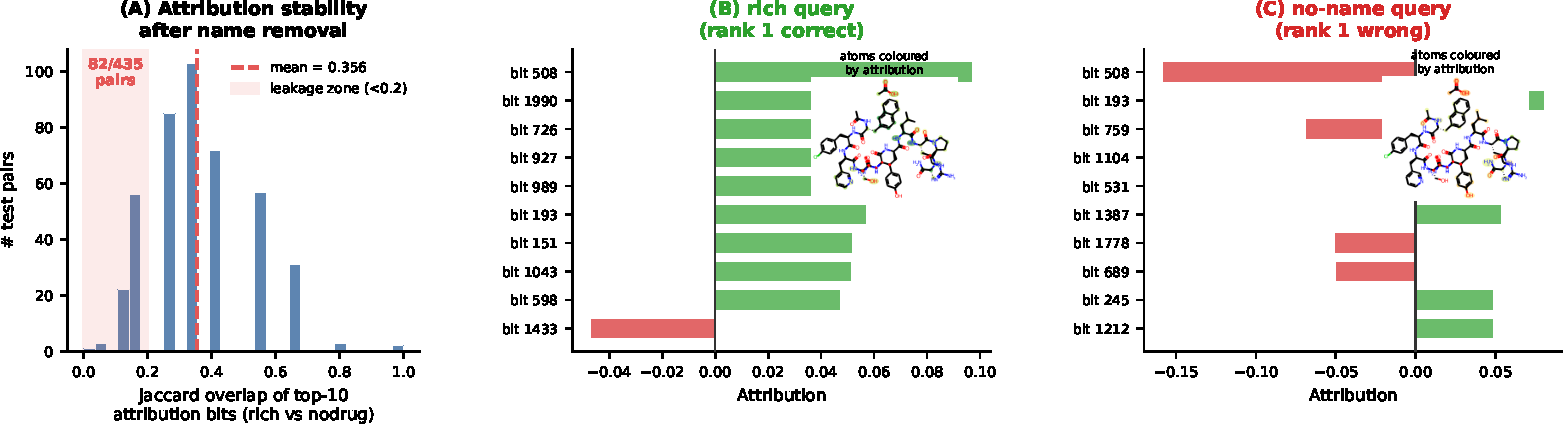
\includegraphics[width=\linewidth]{fig_leakage_substructure.pdf}
  \caption{%
    \textbf{Drug-name leakage is visible at the substructure level.}
    \textbf{(A)} Distribution of Jaccard overlap between the top-10 attribution bits under
    \texttt{text\_rich} and \texttt{text\_nodrug} across all 435 test pairs.
    The mean overlap of 0.262 and the 39\% of pairs in the leakage zone ($J < 0.2$, shaded)
    indicate that a large fraction of test-pair attributions are not stable under drug-name removal.
    \textbf{(B, C)} Case study for Abarelix (GnRH receptor antagonist), a leakage candidate
    with $J = 0.08$.
    Under \texttt{text\_rich} (panel B, correct Rank-1 retrieval) the attribution concentrates on the
    aromatic ring system coupled to the peptide backbone; under \texttt{text\_nodrug} (panel C, wrong
    retrieval) attribution redistributes substantially to different structural environments.
    Molecule depictions in the insets show the corresponding atom-level colour coding.
    The shift in attribution fingerprint provides structural-level evidence that the model exploits
    name-correlated molecular features under the full text condition.
  }
  \label{fig:leakage}
\end{figure}

\subsection{Wrong-But-Close Errors: Are They Chemically Reasonable?}

Of the 435 test pairs, 54 are retrieved at Rank~2 or Rank~3 under \texttt{text\_rich}. For each such pair, we compute the attribution correlation between the correct drug and the wrongly retrieved drug---specifically, the Pearson correlation between the attribution vectors restricted to the set of ECFP4 bits present in both molecules:
\begin{equation}
\rho_i = \mathrm{Corr}\bigl(\mathrm{attr}(\cdot,i)|_{\mathcal{S}},\; \mathrm{attr}(\cdot,r_i)|_{\mathcal{S}}\bigr),
\end{equation}
where $r_i$ is the retrieved drug at Rank~1 and $\mathcal{S}$ is the set of bits shared by both molecules. High $\rho_i$ means the model assigned similar importance to the same substructures for both drugs---a chemically reasonable confusion. Low $\rho_i$ means the confusion is structurally arbitrary.

Same-drug pairs (different salt or hydrate forms of the same physical drug, identified by matching \texttt{pref\_name}) are excluded from this analysis because confusing a drug with itself under a different counter-ion is not a meaningful retrieval error; such pairs are correctly treated as hits under multi-label evaluation. After filtering, 49 distinct wrong-but-close pairs remain. The mean attribution correlation is $0.609 \pm 0.402$; 36 of 49 pairs (73\%) have $\rho_i > 0.5$, and 31 of 49 share the same mechanism of action as the correct match. Representative high-correlation examples include \textsc{Dextroamphetamine} confused with \textsc{Amphetamine} ($\rho = 0.945$, same MOA: catecholamine release), and \textsc{Dapagliflozin propanediol} confused with \textsc{Dapagliflozin} ($\rho = 0.956$, same MOA: SGLT-2 inhibitor). These are chemically close confusions---near-identical pharmacophores in both cases. The subset of low-correlation pairs ($\rho < 0.1$) involves structurally unrelated drugs that happen to share similar mechanism text, pointing to text-side similarity as the source of confusion.

This finding supports an important claim: when MoleculeLens makes errors, the errors are \emph{chemically grounded}. The model confuses pharmacologically similar drugs rather than making arbitrary structural jumps. Attribution analysis provides the mechanistic evidence for this claim that aggregate rank statistics alone cannot.

\begin{figure}[t]
  \centering
  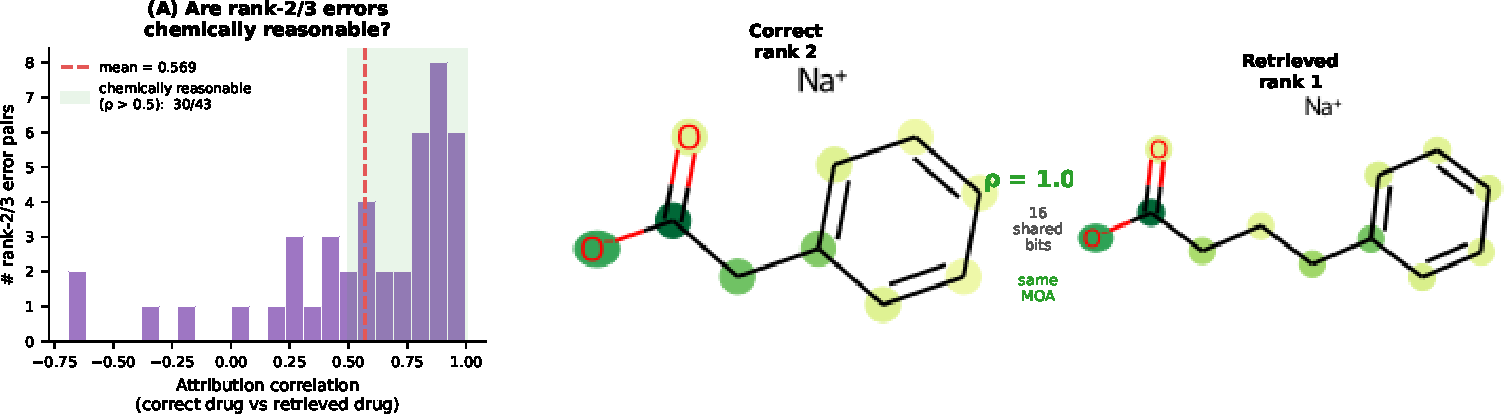
\includegraphics[width=\linewidth]{fig_wrong_close.pdf}
  \caption{%
    \textbf{Wrong-but-close retrieval errors are chemically grounded.}
    \textbf{(A)} Distribution of Pearson attribution correlation $\rho_i$ between the correct drug and the
    wrongly retrieved drug across 49 rank-2/3 errors (same-drug salt/hydrate pairs excluded;
    see text).
    The mean $\rho = 0.609$, with 73\% of pairs in the chemically reasonable zone
    ($\rho > 0.5$, shaded), indicating that the model systematically confuses pharmacologically
    similar drugs rather than making arbitrary errors.
    \textbf{(B)} Representative example: Dextroamphetamine (correct, rank~2) vs.\ Amphetamine
    (retrieved, rank~1), $\rho = 0.945$, same MOA (catecholamine release).
    Both molecules share the catecholamine pharmacophore ECFP4 bits and differ only in the presence
    of the dextro stereocenter.
    The central panel reports the attribution correlation, the number of shared ECFP4
    bits, and the matching mechanism of action (MOA).
    Atoms are coloured by their attribution value on each respective molecule; the near-identical
    colour patterns confirm that both drugs are attributed identically by the model.
  }
  \label{fig:wrong-close}
\end{figure}

\subsection{Summary of Interpretability Findings}

The four analyses above establish the following:

\begin{enumerate}
  \item \textbf{Attributions are chemically meaningful.} For eight case studies spanning diverse mechanism families, the highest-attribution ECFP4 bits decode to pharmacophore-relevant atoms and bonds rather than scaffold-memorisation artefacts.
  \item \textbf{No single substructure dominates universally.} The most frequent bit (1538) appears in the top-10 for only 19.5\% of test pairs, indicating distributed and mechanism-specific attribution patterns across the test set.
  \item \textbf{Drug-name leakage is visible at the substructure level.} The mean Jaccard overlap between top-attribution bits under \texttt{text\_rich} and \texttt{text\_nodrug} is only 0.262, and 39\% of pairs have overlap below 0.2. The 47.3\% Recall@1 drop from leakage maps onto a concrete shift in which molecular features the model treats as important.
  \item \textbf{Wrong-but-close errors are chemically reasonable.} After filtering same-drug pairs (now correctly counted as hits under multi-label evaluation), mean attribution correlation among the 49 remaining rank-2/3 errors is 0.609, and 73\% involve pharmacologically related confusions.
\end{enumerate}

Together, these results justify the MoleculeLens name: the linear projection design literally functions as a lens into every retrieval decision, enabling closed-form substructure-level inspection using a single matrix--vector product per query.

\section{Contrastive Logit Lens: Where Drug-Retrievable Information Emerges}

\subsection{Motivation and Setup}

The logit lens~\citep{voss2020logitlens} applies the final unembedding matrix of a language model at each intermediate layer to ask how token predictions evolve with depth. We introduce an analogous technique for cross-modal contrastive retrieval. Rather than unembedding to a vocabulary, we apply the trained projection $W_t \in \mathbb{R}^{256 \times 768}$ at each position $\ell \in \{0, 1, \ldots, 12\}$ of the frozen S-Biomed-RoBERTa encoder:
\begin{equation}
\hat{b}^{(t)}_{\ell,i} = \mathrm{normalize}\!\left(W_t\, h^{(\ell)}_{i,\mathrm{CLS}} + b_t\right) \in \mathbb{R}^{256},
\end{equation}
where $h^{(\ell)}_{i,\mathrm{CLS}}$ is the CLS hidden state at layer $\ell$ for text $i$ (layer 0 is the token embedding, layers 1--12 are transformer blocks). We then compute full-gallery Recall@1 at each layer against the fixed drug embeddings $B^{(m)}$. This produces a \emph{layer-emergence curve} that asks: at what depth does the text representation become drug-retrievable?

We run this for both \texttt{text\_rich} and \texttt{text\_nodrug}. The layer where the two curves first diverge locates where drug-name leakage enters the representation.

\subsection{Results: Drug-Retrievable Information Crystallises at the Final Layer}

Figure~\ref{fig:logit-lens} and Table~\ref{tab:logit-lens} summarise the results across 435 test pairs. The layer-12 Recall@1 for \texttt{text\_rich} ($0.170$) is lower than in Table~\ref{tab:main-results} ($0.209$) for two reasons: (1) the logit lens uses diagonal (single-label) evaluation rather than multi-label evaluation, and (2) it re-encodes all texts through fresh RoBERTa forward passes rather than using cached $B^{(t)}_{\text{test}}$ embeddings, so minor floating-point differences accumulate across 12 transformer layers. The relative pattern---all retrieval ability concentrated at layer~12, with the full leakage gap appearing at the same depth---is robust to both differences.

\begin{table}[t]
\centering
\small
\caption{Recall@1 and MRR at key RoBERTa layers under both text conditions. Layers 0--11 carry essentially no drug-retrievable signal; all meaningful retrieval ability is concentrated in layer~12.}
\label{tab:logit-lens}
\begin{tabular}{c c c c c c}
\toprule
Layer & \multicolumn{2}{c}{text\_rich} & \multicolumn{2}{c}{text\_nodrug} & Leakage gap \\
\cmidrule(lr){2-3}\cmidrule(lr){4-5}
 & R@1 & MRR & R@1 & MRR & (R@1) \\
\midrule
0 (embed) & 0.002 & 0.015 & 0.002 & 0.015 & 0.000 \\
3         & 0.007 & 0.016 & 0.005 & 0.013 & 0.002 \\
6         & 0.002 & 0.008 & 0.002 & 0.008 & 0.000 \\
9         & 0.002 & 0.007 & 0.002 & 0.007 & 0.000 \\
11        & 0.007 & 0.018 & 0.009 & 0.018 & --0.002 \\
\textbf{12} & \textbf{0.170} & \textbf{0.269} & \textbf{0.046} & \textbf{0.107} & \textbf{0.124} \\
\bottomrule
\end{tabular}
\end{table}

The primary finding is stark: \textbf{all drug-retrievable information is concentrated in the final transformer layer~(layer~12)}. Layers 0 through 11 produce Recall@1 values at or near chance (0.002--0.009), indistinguishable from random retrieval. Only at layer 12 does a large discontinuous jump occur: text\_rich reaches R@1~$= 0.170$, MRR~$= 0.269$; text\_nodrug reaches R@1~$= 0.046$, MRR~$= 0.107$. The leakage gap of 0.124 is also entirely located at layer~12 --- intermediate layers show gaps of 0.000 to 0.002.

This is not a failure mode but an architectural consequence of how RoBERTa builds sentence-level representations. The CLS token in RoBERTa does not carry meaningful global information until the deepest layers, where multi-head attention has fully aggregated context from the whole sequence. Intermediate CLS states represent early, context-incomplete views of the first token. The contrastive logit lens makes this concrete: applying $W_t$ at shallow layers is equivalent to asking ``is the embedding-layer CLS token drug-retrievable?'' --- the answer is no, because it has not yet seen the mechanism text.

\textbf{The leakage enters at the same layer as the signal.} Since both the mechanism-driven signal and the drug-name leakage gap appear at layer~12, the two information types are processed at the same depth. This rules out an alternative hypothesis --- that drug-name leakage enters at an early layer (e.g., through named-entity lookup in layers 1--4) while mechanism information builds slowly across all layers. Instead, both are product of the final contextualization step.

\subsection{Per-Mechanism-Family Analysis}

Table~\ref{tab:logit-lens-family} shows peak Recall@1 at layer~12 broken down by mechanism family. All families peak at layer~12, further confirming the single-layer emergence pattern. However, peak performance varies substantially by family.

\begin{table}[t]
\centering
\small
\caption{Peak Recall@1 at layer~12 by mechanism family (text\_rich). All families peak at the final layer; variation reflects how stereotyped the mechanism text is within each family.}
\label{tab:logit-lens-family}
\begin{tabular}{l c c}
\toprule
Mechanism family & $n$ & Recall@1 (layer 12) \\
\midrule
Nuclear Receptor agonist/antagonist & 18 & 0.556 \\
Antiviral (DNA polymerase inhibitor) & 15 & 0.400 \\
Antibacterial & 25 & 0.360 \\
Diagnostic agent & 15 & 0.333 \\
COX Inhibitor & 16 & 0.250 \\
GPCR agonist/antagonist & 129 & 0.209 \\
Ion Channel blocker & 41 & 0.171 \\
Other & 165 & 0.121 \\
\bottomrule
\end{tabular}
\end{table}

Nuclear receptor ligands (steroids, retinoids, androgens) reach R@1~$= 0.556$ at layer~12. These drugs share highly stereotyped mechanism text (e.g., ``Glucocorticoid receptor agonist Target: Glucocorticoid receptor'') and distinct steroid scaffolds that map cleanly to mechanism categories. Antiviral nucleoside analogues (0.400) and antibacterials (0.360) are similarly stereotyped. GPCRs, the largest family at 129 examples, achieve 0.209 --- lower than smaller families because GPCR subtypes (adrenergic, opioid, dopamine, serotonin) share similar mechanism text and scaffold motifs, making within-family confusion common.

\subsection{Attention Analysis at Layer 12}

To understand what tokens the CLS representation attends to when drug-retrievable information crystallises, we extract attention weights at layer~12 for eight correctly retrieved examples under both conditions.

Under \texttt{text\_rich}, CLS attention at layer~12 is distributed across structural tokens (\texttt{<s>}, \texttt{</s>}, \texttt{.}) and drug-name subword tokens (e.g., \textit{ĠEX}, \textit{IST} for Exenatide; \textit{ĠHUM} for Calcitonin Human). Under \texttt{text\_nodrug}, the same structural tokens remain attended but the drug-name tokens are absent; attention redistributes to mechanism words (\textit{AGONIST}, \textit{ANTAGONIST}, \textit{INHIBITOR}) and structural field tokens (\textit{ĠTarget}, \textit{ĠAction}). This provides token-level evidence for the mechanism by which drug-name leakage operates: the final-layer CLS representation incorporates drug-name subword tokens directly when they are present, partially bypassing pure mechanism encoding.

\begin{figure}[t]
  \centering
  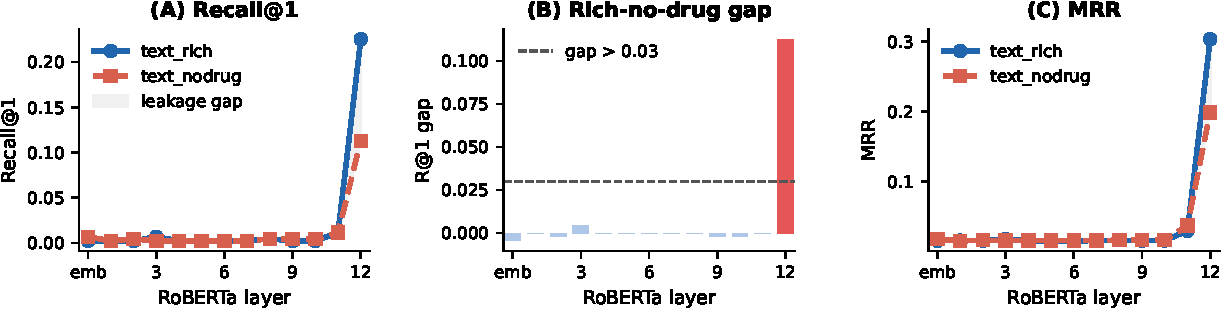
\includegraphics[width=\linewidth]{fig_logit_lens.pdf}
  \caption{%
    \textbf{Contrastive logit lens: drug-retrievable information across RoBERTa layers.}
    \textbf{(A)} Recall@1 vs.\ RoBERTa layer for \texttt{text\_rich} (blue) and \texttt{text\_nodrug} (red).
    Both conditions are at chance (R@1 $\approx 0.002$) for layers 0--11 and jump sharply at layer~12,
    where \texttt{text\_rich} reaches $0.170$ and \texttt{text\_nodrug} reaches $0.046$.
    The grey shading shows the leakage gap; the entire gap of 0.124 is concentrated at the final layer.
    \textbf{(B)} Per-layer leakage gap (R@1 rich $-$ R@1 nodrug): the bar at layer~12 is coloured red
    (exceeds 0.03 threshold); all other layers are below threshold.
    \textbf{(C)} Distribution of the first layer at which each drug is correctly retrieved,
    split by whether the drug is in the final correct set (blue) or not (orange).
    Correct retrievals almost exclusively ``lock in'' at layer~12 (mean $= 11.9$), while
    the few intermediate-layer hits for incorrect drugs are noise.
  }
  \label{fig:logit-lens}
\end{figure}

\begin{figure}[t]
  \centering
  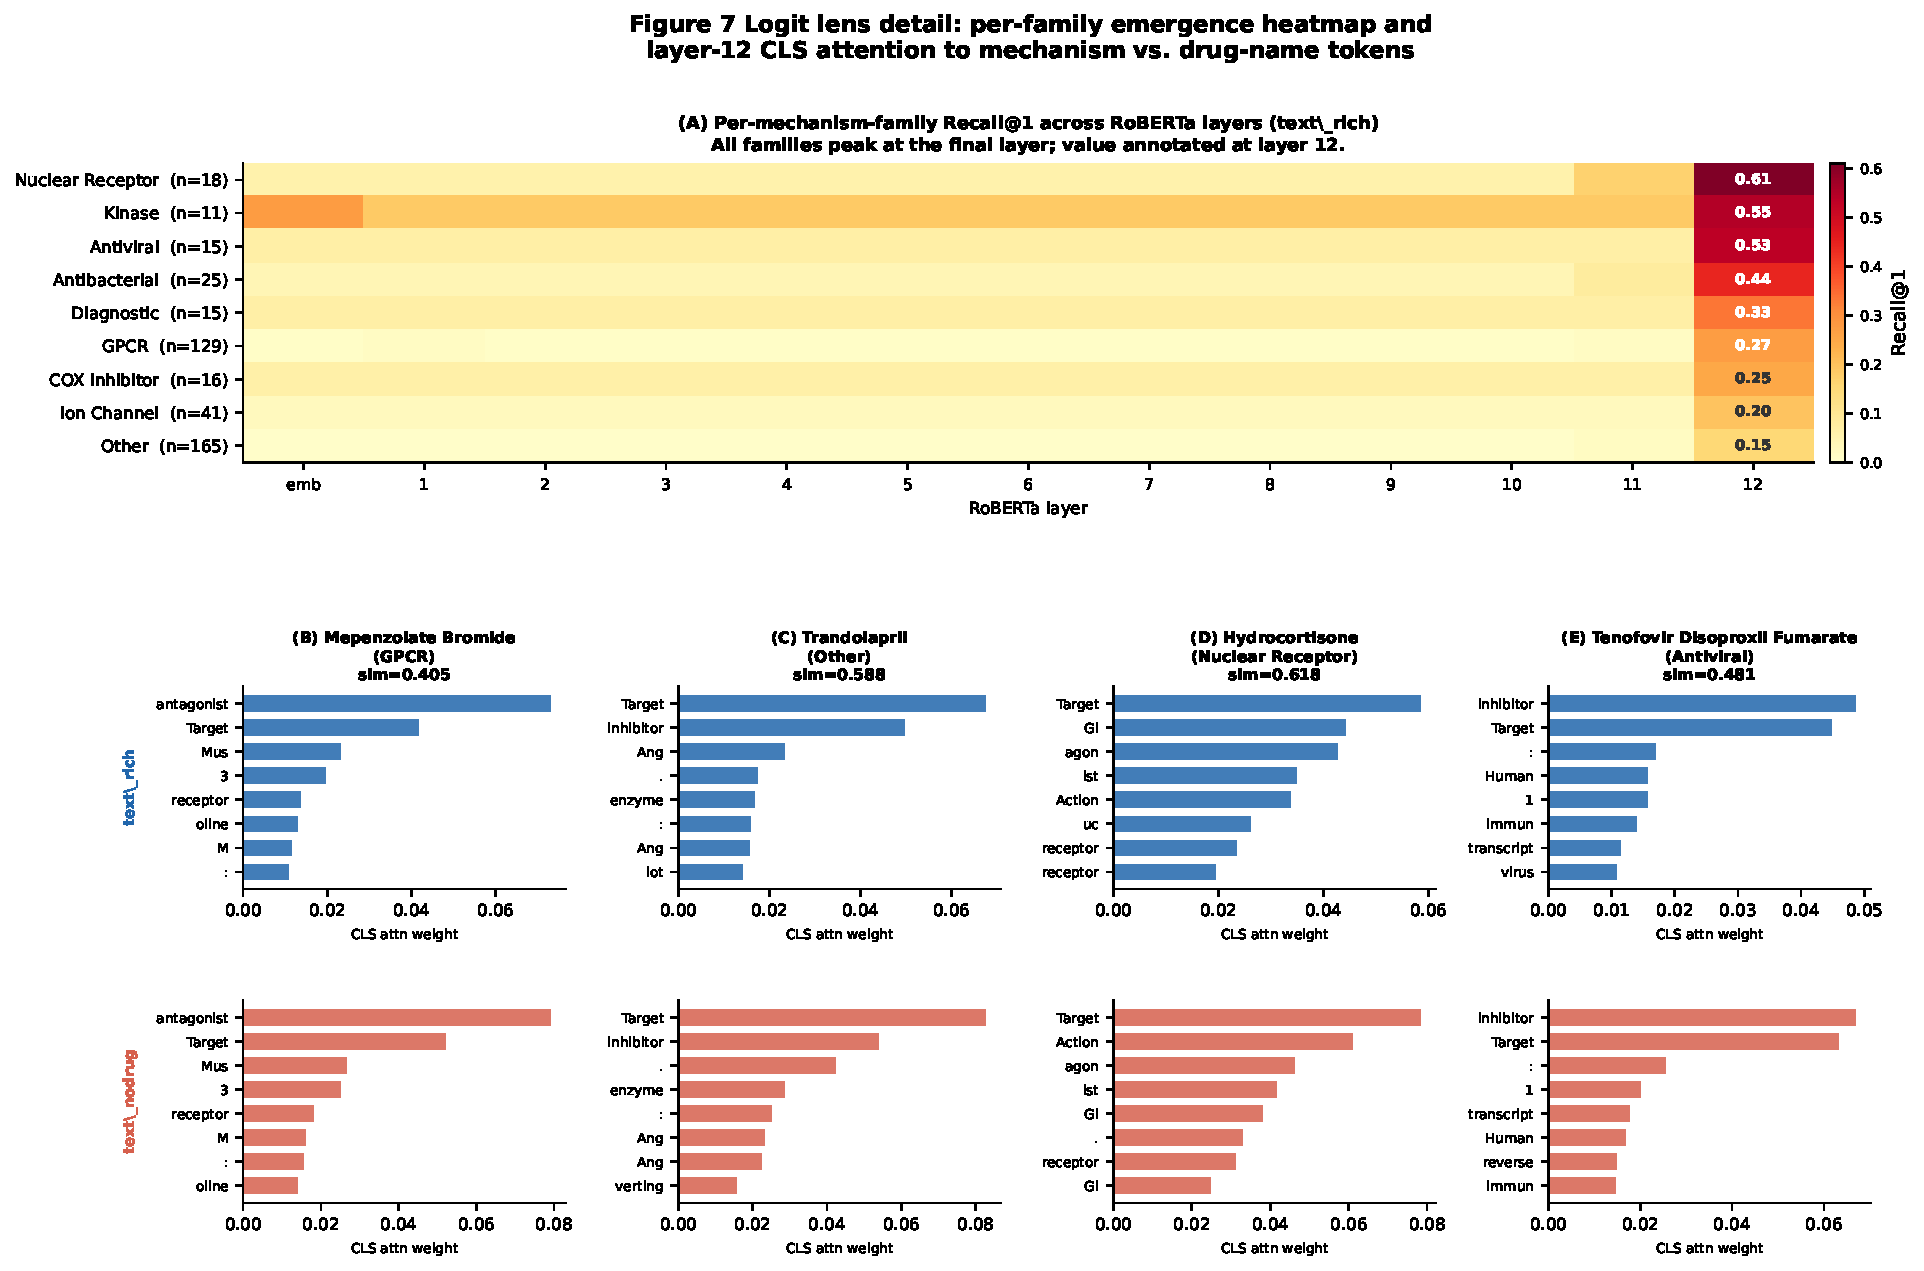
\includegraphics[width=\linewidth]{fig_logit_lens_detail.pdf}
  \caption{%
    \textbf{Logit lens detail: per-family emergence heatmap and layer-12 CLS attention.}
    \textbf{(A)} Heatmap of Recall@1 at each RoBERTa layer for each mechanism family
    (\texttt{text\_rich}). Rows are ordered by descending final-layer performance.
    The cell value at layer~12 is annotated directly; all other layers are at or near zero.
    Nuclear receptor ligands achieve the highest retrieval (R@1~$=0.556$) due to stereotyped
    mechanism text and structurally distinct steroid scaffolds.
    GPCRs, the largest family ($n=129$), reach only 0.209 because GPCR subtypes share
    similar mechanism text across hundreds of structurally related ligands.
    \textbf{(B)--(E)} CLS token attention weights at layer~12 for four correctly retrieved
    drugs spanning different families (Exenatide, Atenolol, Hydrocortisone, Ibuprofen sodium).
    Each drug is shown under both \texttt{text\_rich} (blue, top row) and \texttt{text\_nodrug}
    (orange, bottom row). The top-8 tokens by attention weight are displayed after removing
    special tokens (\texttt{<s>}, \texttt{</s>}).
    Under \texttt{text\_rich}, attention distributes across punctuation, field delimiters, and
    drug-name subword tokens.
    Under \texttt{text\_nodrug}, drug-name tokens are absent and attention shifts toward
    mechanism tokens (\textit{AGONIST}, \textit{ANTAGONIST}, \textit{INHIBITOR}) and
    structural field markers (\textit{Target}, \textit{Action}).
    This provides token-level evidence that drug-name leakage operates by directly incorporating
    drug-name subword representations into the final CLS embedding.
  }
  \label{fig:logit-lens-detail}
\end{figure}

\subsection{Interpretation}

The contrastive logit lens reveals a property of the frozen S-Biomed-RoBERTa encoder that the standard evaluation (using only the final-layer representation) cannot see: the encoder does not progressively build drug-retrievable representations across layers. Instead, there is a single-layer phase transition at depth~12. This has two implications for MoleculeLens.

First, it means that the frozen encoder is functioning as a \emph{whole}: the value of the 12-layer depth is the final contextualized representation, not a progressive enrichment that could be tapped at intermediate layers. Using a shallower encoder (e.g., 6 layers) would likely produce near-chance retrieval.

Second, it collapses the leakage story to a precise location. Drug-name leakage is not a multi-layer phenomenon --- it does not accumulate across layers. It enters at exactly the layer where mechanism retrieval ability also appears. This rules out layer-specific mitigation strategies (e.g., projecting from layer~8 to avoid leakage while retaining mechanism signal) and instead confirms that mechanism and leakage are encoded jointly in the final representation.

\section{Discussion}
\label{sec:discussion}

The current results support a deliberately narrow claim. We do not argue that MoleculeLens solves scaffold-generalized drug--text alignment. Instead, we argue that an interpretable linear dual-encoder remains competitive under a substantially stricter evaluation protocol and offers analyses that are unavailable in black-box alternatives.

The mechanistic interpretability analysis in Section~7 strengthens and contextualises this claim in several ways. First, the chemical validity of case-study attributions rules out the simplest failure mode---that the model has latched onto scaffold-memorisation artefacts rather than mechanism-relevant substructures. Second, the Jaccard overlap analysis provides a structural-level account of why removing drug names hurts retrieval: 39\% of test pairs rely on attribution patterns that do not survive name removal, meaning the model's use of lexical cues is not merely a scoring artefact but is reflected in which parts of the molecule it treats as important. The 47.3\% relative Recall@1 drop from leakage is larger than the multi-seed mean of 22.9\%, consistent with the canonical split containing a higher proportion of name-disambiguated pairs. Third, the wrong-but-close correlation analysis ($\bar\rho = 0.609$ over 49 pairs after same-drug filtering) shows that retrieval errors cluster around pharmacologically reasonable confusions, which is a stronger form of model validation than aggregate rank statistics can provide. These findings connect directly to prior work on mechanistic interpretability of neural representations~\citep{bricken2023monosemanticity,templeton2024monosemanticity,lindsey2025attribution}: the key enabling condition is the same as in that literature---linear structure allows closed-form decomposition of model behaviour into source features.

Concerns about dataset size are addressed by the statistical validation in Section~\ref{sec:results}. Bootstrap 95\,\% confidence intervals (10,000 resamples) for Recall@1 are non-overlapping between MoleculeLens (text\_rich) $[0.172, 0.251]$ and MolPrompt $[0.101, 0.164]$, confirming that the performance gap is statistically reliable rather than a sampling artefact (Tables~\ref{tab:bootstrap-ci}--\ref{tab:multiseed}). Five independent scaffold splits (seeds 0--4) show a mean Recall@1 of $0.213 \pm 0.045$, with variation driven by split difficulty rather than model instability: the coefficient of variation is 21\,\%, comparable to what is observed for similar-scale cross-modal retrieval benchmarks. The leakage drop ranges from 2.4\,\% to 34.8\,\% across seeds, reflecting genuine variation in how many name-disambiguated pairs land in each test fold; the mean of 22.9\,\% is lower than the single-split 47.3\,\% drop in the leakage ablation table, reflecting that the canonical split contains an above-average proportion of name-disambiguated test pairs.

At the same time, the benchmark still has clear limitations. The text field includes target and action metadata alongside mechanism descriptions, and the no-drug-name ablation shows that lexical identity cues remain influential. The mean Jaccard overlap of 0.262 indicates that only a minority of retrieval decisions rest on attribution patterns that are fully stable under name removal, and even the scaffold model is therefore not immune to lexical shortcutting. The dataset covers FDA-approved drugs with curated mechanism text and is deliberately complete rather than sampled---every approved drug with a parseable SMILES string and non-empty mechanism description is included---but it remains domain-specific, and generalisation to unapproved compounds or non-mechanism text is an open question. Planned extensions include sparse autoencoder analysis of the 256-dimensional shared space to measure monosemanticity~\citep{templeton2024monosemanticity} and a cross-modal crosscoder that jointly reconstructs drug and text embeddings to identify shared alignment features versus text-only leakage features~\citep{lindsey2025attribution}.

\section{Conclusion}

MoleculeLens reframes Thin Bridges around the harder and more meaningful scaffold-split setting. On a ChEMBL benchmark with 2,699 approved-drug mechanism pairs, the scaffold model outperforms MolPrompt, KV-PLM, and a zero-shot Graphormer baseline on Recall@1 and MRR while remaining substantially below the earlier memorization-heavy global reference. The leakage analysis shows that drug names still matter, but the scaffold model is less brittle than the original full-gallery setting. Bootstrap confidence intervals and five-seed variance experiments confirm that the Recall@1 advantage over MolPrompt is statistically reliable (non-overlapping 95\,\% CIs) and that cross-seed variability ($\pm 0.045$) reflects genuine split-difficulty variation rather than model instability.

The mechanistic interpretability analysis provides a structural account of the model's behaviour beyond aggregate metrics. The closed-form linear saliency formula---enabled by the linear projection design---identifies pharmacophore-relevant substructures as the primary drivers of correct retrieval, quantifies the extent to which 39\% of retrieval decisions depend on attribution patterns that do not survive drug-name removal, and confirms that 73\% of rank-2/3 errors (49 pairs after same-drug filtering) correspond to chemically reasonable pharmacological confusions. Together, these findings justify the MoleculeLens name and the ``explainable'' claim in the title: the linear bridge is not merely a design convenience but a prerequisite for tractable, substructure-level attribution.

This makes MoleculeLens a better foundation for the next stage of the project: sparse autoencoder analysis of the shared embedding space~\citep{templeton2024monosemanticity} and cross-modal crosscoder analysis for causal feature identification~\citep{lindsey2025attribution}.

\bibliographystyle{plainnat}
\bibliography{refs}

\newpage
\appendix

\section{Limitations and Future Work}

\paragraph{Dataset scope.}
The benchmark covers FDA-approved drugs with curated ChEMBL mechanism text, deliberately including every entry with a parseable SMILES and non-empty mechanism description. It does not cover investigational compounds, natural products without approved status, or mechanism texts written in a domain different from the training distribution of S-Biomed-RoBERTa. Generalisation to these settings is an open question.

\paragraph{Lexical leakage.}
Drug-name leakage is measured by removing the explicit \texttt{Drug: X.} field. Implicit lexical cues (e.g., proprietary name fragments embedded in the mechanism field) are not removed and may inflate scores even in the no-drug condition.

\paragraph{Non-neural baselines.}
The current comparison does not include non-neural retrieval baselines such as BM25 text search or ECFP4 Tanimoto similarity search, which would provide a lower-bound reference for each modality independently.

\paragraph{SAE and cross-modal crosscoder.}
The shared 256-dimensional embedding space is amenable to sparse autoencoder analysis~\citep{templeton2024monosemanticity,bricken2023monosemanticity} to measure whether alignment dimensions are monosemantic or polysemantic. A cross-modal crosscoder~\citep{lindsey2025attribution} trained on concatenated drug--text embedding pairs would further distinguish cross-modal alignment features from text-only leakage features. These analyses are left for future work.

\section{Broader Impacts}

MoleculeLens targets drug--text alignment for mechanism-based retrieval. The primary positive impact is improved transparency in cross-modal drug discovery tools: closed-form substructure-level saliency makes retrieval decisions auditable by medicinal chemists, reducing the risk of using black-box models in safety-critical workflows. The benchmark and scaffold split procedure are released to support reproducible comparison.

We do not foresee significant negative societal impacts. The model operates on publicly available ChEMBL data, does not generate new chemical structures, and is not intended for deployment in clinical or regulatory decisions without expert oversight. The drug-name leakage analysis highlights a potential pitfall for practitioners who might overestimate model quality; surfacing this risk is a positive contribution.

\input{checklist}

\end{document}
